\documentclass[11pt,letterpaper]{article}
\usepackage[T1]{fontenc}
\usepackage{lmodern,microtype}
\usepackage[margin=0.85in]{geometry}
\usepackage{amsmath,amssymb,mathtools,booktabs,tabularx,array,enumitem}
\usepackage{xcolor,tikz,fancyhdr}
\usepackage[colorlinks=true,linkcolor=blue!45!black,citecolor=blue!45!black,urlcolor=blue!45!black]{hyperref}
\usepackage{xurl}
\hypersetup{pdftitle={Adaptive path refinement for quadform geodesics},pdfauthor={Method proposal based on Pawel Gajer\textquotesingle s local-disk construction}}
\usetikzlibrary{arrows.meta,calc}
\definecolor{ink}{HTML}{17354A}
\definecolor{accent}{HTML}{217C82}
\setlength{\parindent}{0pt}
\setlength{\parskip}{6pt}
\setlist{nosep,leftmargin=1.5em,topsep=4pt}
\setlength{\emergencystretch}{2em}
\pagestyle{fancy}
\fancyhf{}
\fancyhead[L]{\small\color{ink}Quadform geodesics: refinement proposal}
\fancyhead[R]{\small September 2026}
\fancyfoot[L]{\small Method specification; no solver results}
\fancyfoot[R]{\thepage}
\setlength{\headheight}{14pt}
\newcommand{\R}{\mathbb{R}}
\newcommand{\norm}[1]{\left\lVert#1\right\rVert}
\newcommand{\dd}{\,\mathrm{d}}
\newcommand{\src}[1]{\nolinkurl{#1}}
\title{\color{ink}\textbf{Adaptive path refinement for quadform geodesics}\\[5pt]\large Surface-valid connectors, local sampling, and alternative refinements}
\author{Method proposal based on Pawel Gajer's local-disk construction}
\date{\input{build/refinement_timestamp.tex}}
\begin{document}
\maketitle
\thispagestyle{fancy}
\begin{abstract}
\noindent Local sampling proposes shorter replacements between fixed points of a path on a quadratic surface. Every graph edge measures a specified curve \emph{on the surface}. Retaining the old route makes shortening monotone in exact arithmetic, but local stagnation does not establish global optimality. The main text preserves the original grid-based proposal, and Appendix~\ref{app:three-point} preserves the subsequent R configuration. Appendix~\ref{app:cpp-current} specifies the current package-integrated C++ configuration, including analytic connector lengths and all three neighborhood rules. This document specifies algorithms; it reports no numerical experiment results.
\end{abstract}

\textbf{Version and precedence.} For the implementation identified by
\src{self-contained-cpp-analytic-v3}, Appendix~\ref{app:cpp-current} is the
current operational specification. Earlier sections remain historical
alternatives, not additional requirements imposed on that configuration.
In particular, their grid, PCG64, checkpoint, publication and quadrature
protocols must not be combined with the current algorithm. Identifying a
behavior here does not establish that the implementation satisfies it.

\section{The distance being estimated}
Let $D$ be a closed unit disk or the square $[0,1]^2$, and let
\begin{equation}\label{eq:surface}
 F(u)=\bigl(u,f(u)\bigr),\qquad f(u)=u^T A u,\qquad u\in D,\quad A=A^T\in\R^{2\times2}.
\end{equation}
There is no implicit factor of $1/2$. An isotropic paraboloid has $A=cI$, $c>0$; a saddle can have $A=\operatorname{diag}(c,-c)$. Given exact parameter endpoints $a,b\in D$, the target is
\begin{equation}\label{eq:distance}
 d_D(a,b)=\inf_{u}\int_0^1\sqrt{\dot u(t)^T M(u(t))\dot u(t)}\dd t,
 \qquad M(u)=I+4(Au)(Au)^T,
\end{equation}
where the infimum is over absolutely continuous paths in $D$ with $u(0)=a$ and $u(1)=b$. The corresponding surface endpoints are $F(a),F(b)$.

The domain is part of the problem. Paths may touch its boundary. A shortest path on the unrestricted quadform need not solve the restricted problem if it leaves $D$. The domain must not be replaced by a point sample's convex hull. Other balls and boxes in the shared fixtures retain their own declared coordinates and sizes; they are not silently rescaled to the unit disk or unit square.

\textbf{Historical first proposal.} Use exact surface connectors, the user's two-disk sampling regions, and sequential single-vertex replacement as a simple baseline. Add the full local-graph replacement as a separate configuration, followed by larger windows if local moves stall. Keep the best feasible path and its diagnostics after every accepted update. The current configuration is specified separately in Appendix~\ref{app:cpp-current}.

\clearpage
\section{An edge must represent a curve on the surface}
For parameter points $a,b$, set $\delta=b-a$. Define the edge to be the lifted straight parameter segment
\begin{equation}\label{eq:connector}
 \gamma_{ab}(t)=F(a+t\delta),\quad 0\le t\le1,
 \qquad w(a,b)=\int_0^1\sqrt{\norm{\delta}^2+
 \bigl[2(a+t\delta)^TA\delta\bigr]^2}\dd t.
\end{equation}
Both proposed domains are convex, so the entire parameter segment stays in $D$. Thus each edge, and every concatenation of edges, is feasible. The edge is generally \emph{not} itself a geodesic. Its length is known from a one-dimensional integral even when the shortest surface path is unknown.

Using $\norm{F(a)-F(b)}$ instead would measure a straight ambient chord. That chord generally leaves the surface. In a complete graph with chord weights, the direct endpoint edge is already shortest by the Euclidean triangle inequality; adding samples cannot recover the missing curvature.

\subsection{Closed form for a single quadratic height}
Write $s=\norm{\delta}$, $\alpha=2a^TA\delta$, and $\beta=2\delta^TA\delta$. For $s>0$, define
\begin{align}
 H_s(v)&=\tfrac12\left[v\sqrt{s^2+v^2}+s^2\operatorname{arsinh}(v/s)\right],\\
 w(a,b)&=\begin{cases}
 [H_s(\alpha+\beta)-H_s(\alpha)]/\beta,&\beta\ne0,\\
 \sqrt{s^2+\alpha^2},&\beta=0.
 \end{cases}\label{eq:closed}
\end{align}
For $a=b$, return zero directly. This formula follows by integrating $\sqrt{s^2+(\alpha+\beta t)^2}$. A small nonzero $\beta$ can cause cancellation in the difference of antiderivatives. A stable evaluation needs scale-aware error control. Ordinary adaptive quadrature is not a sufficient safeguard against a narrow unsampled minimum. Appendix~\ref{app:cpp-current} specifies the current analytic evaluation. Replacing a small denominator by an arbitrary floor changes the mathematical quantity.

\subsection{Connection to the existing geometry utilities}
The current \src{geosmooth} implementation provides \src{quadform.metric()} and \src{edge.lengths.synthetic.geometry()} in \src{R/synthetic_geometry.R}. The latter integrates lifted parameter segments numerically and handles identical endpoints. Its small-coefficient shortcut and quadrature tolerances still require dedicated validation across the fixture scales; the API name does not certify numerical error.

For the fixture convention $F(u)=Q(u,u^TA_1u,\ldots,u^TA_mu)+o$, with $Q^TQ=I$, the same construction gives
\begin{equation}\label{eq:general}
 M(u)=I+4\sum_{j=1}^m(A_ju)(A_ju)^T,\qquad
 w(a,b)=\int_0^1\sqrt{\norm{\delta}^2+\sum_{j=1}^m(\alpha_j+\beta_jt)^2}\dd t.
\end{equation}
An ambient isometry or translation does not change these lengths. Equation~\eqref{eq:general} supports higher-dimensional extensions, but this proposal's first solver scope is two parameter dimensions with one height function.

\clearpage
\section{Grid initialization and the proposed sampling regions}
Construct a regular parameter grid with spacing $h$, retain points in $D$, and add the exact endpoints as vertices. Weight all allowed edges by \eqref{eq:connector}. Declare the grid stencil and endpoint attachment rule explicitly. A practical initializer attaches each endpoint to several nearby grid vertices, and includes the direct lifted endpoint connector as a feasible fallback. Run an undirected shortest-path algorithm and retain the better feasible route.

A disconnected numerical grid is an initialization defect to report or rebuild. The direct connector already gives a valid path in a convex domain. MST repair of a sampled data graph is therefore unnecessary here and would not establish geodesic accuracy.

\textbf{Grid refinement alone is insufficient with a fixed stencil.} On a flat surface, an eight-neighbor square grid from $(0,0)$ to $(1,1/2)$ has length $(1+\sqrt{2})/2\approx1.2071$, versus $\sqrt{5}/2\approx1.1180$ for the straight path, whenever the endpoints lie on the grid. The approximately $7.97\%$ excess persists as compatible grid spacings decrease. Extra directions or off-grid refinement must remove this bias. The direct-connector fallback makes the flat final answer exact, so diagnose the stencil separately rather than treating that flat pass as evidence that local refinement works.

Let $U=(u_0,\ldots,u_m)$ be the current parameter path, with $q_i=F(u_i)$. For an interior vertex, define
\begin{align}
 r_-&=\norm{u_i-u_{i-1}},& S_-&=D\cap B(u_{i-1},r_-),\\
 r_+&=\norm{u_i-u_{i+1}},& S_+&=D\cap B(u_{i+1},r_+).
\end{align}
This interprets the second disk in the original description as centered at $u_{i+1}$. Draw $N$ accepted samples from each clipped disk and form their union $R$. Uniform parameter-area sampling is a proposal distribution; it is not uniform surface-area sampling. Rejection sampling preserves the former distribution; projecting rejected points onto the boundary does not.

\begin{center}
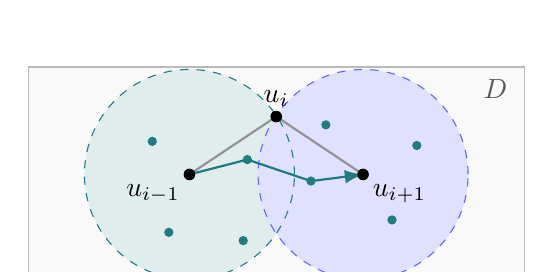
\begin{tikzpicture}[scale=1.05,>=Latex]
 \fill[gray!5] (-3,-1.3) rectangle (3,1.3);
 \draw[gray!55] (-3,-1.3) rectangle (3,1.3);
 \begin{scope}
  \clip (-3,-1.3) rectangle (3,1.3);
  \fill[accent!14] (-1.05,0) circle (1.27);
  \fill[blue!12] (1.05,0) circle (1.27);
  \draw[accent,dashed] (-1.05,0) circle (1.27);
  \draw[blue!60,dashed] (1.05,0) circle (1.27);
 \end{scope}
 \draw[thick,gray!85] (-1.05,0)--(0,.7)--(1.05,0);
 \draw[thick,accent,->] (-1.05,0)--(-.35,.18)--(.42,-.08)--(1.05,0);
 \foreach \x/\y in {-1.5/.4,-1.3/-.7,-.35/.18,.42/-.08,.6/.6,1.4/-.55,1.7/.35,-.4/-.8}
  \fill[accent] (\x,\y) circle (1.6pt);
 \fill (-1.05,0) circle (2pt) node[below left] {$u_{i-1}$};
 \fill (0,.7) circle (2pt) node[above] {$u_i$};
 \fill (1.05,0) circle (2pt) node[below right] {$u_{i+1}$};
 \node[gray!70!black] at (2.65,1.03) {$D$};
\end{tikzpicture}
\end{center}
{\small Schematic in parameter space: old route in gray; a sampled candidate in teal. Every segment is lifted before evaluating length. The pictured candidate is not asserted to be shorter for an unspecified $A$.}

\clearpage
\section{Two explicit local replacement algorithms}
Both variants retain the old feasible route, keep the window endpoints fixed, and compare costs using the same edge evaluator. A local graph path can visit \emph{any subset} of its candidates; it is not required to visit every sampled point.

\subsection{Variant A: replace a single interior vertex}
Choose
\begin{equation}\label{eq:single}
 v_*\in\mathop{\arg\min}_{v\in R\cup\{u_i\}}
 \left[w(u_{i-1},v)+w(v,u_{i+1})\right].
\end{equation}
Also compare the direct edge $w(u_{i-1},u_{i+1})$, which permits removal of $u_i$. Accept the best replacement only if the improvement exceeds the numerical acceptance margin in Section~\ref{sec:stopping}. The candidate evaluations cost $O(N)$ edge computations per window. This is a finite sampled search, not a claim to solve continuous minimization over the disks.

A fixed vertex count restricts the family of curves. When additional resolution is needed, insert the parameter midpoint of an existing edge. Its two lifted subsegments describe exactly the same curve as the original edge, so their exact total length is unchanged. Subsequent moves can bend that refined path. Record numerical discrepancies in this identity rather than accepting them as geometric improvement.

\subsection{Variant B: replace by a path through a local graph}
Construct an undirected graph on $\{u_{i-1},u_i,u_{i+1}\}\cup R$ using surface-valid edges. A complete graph is the simplest unambiguous specification; always retain both old edges and the direct window connector. Find the shortest route from $u_{i-1}$ to $u_{i+1}$ and compare it with the old two-edge route. This can insert several vertices in one step but requires $O(N^2)$ edge evaluations before graph search. A sparse graph is a separate variant with its own connection rule; it must still contain the old route.

\subsection{Sequential sweep and durable state}
\begin{enumerate}
\item Validate the geometry, declared domain, endpoints, and configuration. Return the identity path immediately when the endpoints coincide.
\item Build the initial path and remove exact consecutive duplicates. Subdivide its edges to parameter spacing at most $h$, with at least one interior vertex for distinct endpoints; a direct-connector initializer otherwise has no movable vertex. Independently evaluate and save the incumbent.
\item Select the next window from the \emph{current} path. Generate samples using its current neighbors and the recorded random seed. Apply Variant A or B.
\item Check candidate endpoints, domain feasibility, finite edge costs, and the acceptance inequality. Commit only an accepted replacement; otherwise retain the incumbent.
\item Advance through the path with a bounded work queue. Newly inserted vertices enter the next sweep so one sweep cannot grow indefinitely. Alternate sweep direction or record a randomized ordering.
\item At a sweep boundary, checkpoint the incumbent and diagnostics. Apply the declared stopping and escalation rules. Return the best feasible path even if the refinement budget expires, with an explicit accuracy status.
\end{enumerate}
Overlapping replacements computed from an old path cannot safely be installed simultaneously. The baseline updates sequentially. Parallel proposals require non-overlapping windows and a final joint cost check. Near-coincident but distinct endpoints must not be merged by a coarse deduplication threshold.

\clearpage
\section{Modifications worth comparing}
These are alternative modifications. Section~\ref{sec:protocol} fixes the initial configuration and identifies which options remain off.

\renewcommand{\arraystretch}{1.16}
\begin{tabularx}{\textwidth}{@{}>{\raggedright\arraybackslash}p{0.21\textwidth}>{\raggedright\arraybackslash}X>{\raggedright\arraybackslash}X@{}}
\toprule
Modification & Intended benefit & Limitation or control \\
\midrule
Single-vertex search & Cheap, transparent accepted moves; simple error handling. & Needs insertion and wider windows to escape its restricted path family. \\
Full local graph & Can replace one bend with a multi-vertex detour. & Quadratic edge cost; cap candidate count and path growth. \\
Center or corridor samples & Put more candidates near the movable part of the path. & A narrow corridor may exclude a better route entirely. \\
Longer windows & Allow coordinated changes across several consecutive bends. & More expensive; preserve every edge of the old subpath. \\
Multiple spatial scales & Expand beyond disks whose radii shrink with vertex spacing. & Define radii relative to domain size and local spacing; record the schedule. \\
Deterministic samples & Reduce seed variability and make comparisons reproducible. & Rotate or shift the design; deterministic directional bias can remain. \\
Metric-aware proposals & Balance steps by local surface length rather than parameter length. & A frozen local metric is only an approximation away from its center. \\
Global graph refresh & Reconsider routes outside the current path's corridor. & Larger memory and construction cost; local sampling alone is not global coverage. \\
Continuous polishing & Improve a good discrete route with movable interior coordinates. & Solver degeneracy and local minima require separate safeguards. \\
\bottomrule
\end{tabularx}

\textbf{Sampling changes.} A disk centered at $u_i$, or a tube around the current parameter subpath, can supplement the two endpoint-centered disks. A mixture can reserve samples for a wider region of $D$. Declare mixture weights and accepted sample counts. A separate boundary-sampling component can target boundary-constrained routes. For a metric-aware proposal centered at $c$, sample inside
\[
 \{v:(v-c)^TM(c)(v-c)\le\rho^2\}\cap D.
\]
This ellipse is a proposal region, not a geodesic ball. Randomized low-discrepancy designs are another option; clipping or rejection changes their coverage properties and must be documented.

\textbf{Broader moves.} Replace windows spanning several edges and occasionally recompute a global route on retained samples plus new domain-wide samples. Include old path edges so the incumbent remains available. Retaining nodes without adequate new connections does not ensure improvement. Sparse connection radii and neighbor counts are method parameters, not borrowed guarantees.

\textbf{Path size.} Subdivide long edges to add freedom and remove redundant vertices only when the replacement passes the same cost check. Arbitrary resampling followed by new lifted connectors can change the curve and increase length. A node cap should reject an oversized proposal or invoke a separately checked simplification, never silently truncate it.

\clearpage
\section{What convergence and stopping can establish}\label{sec:stopping}
For exact connector costs and accepted shortening moves, the incumbent lengths satisfy
\begin{equation}\label{eq:monotone}
 d_D(a,b)\le L_{k+1}\le L_k.
\end{equation}
Hence the sequence of lengths converges. This does not prove that its limit is $d_D$, that the path itself converges, or that the shortest path is unique. Finite samples can miss a useful move; short windows can remain trapped; a fixed stencil or narrow corridor can leave systematic error.

This distinction is also present in the sampling-based planning literature: Karaman and Frazzoli prove asymptotic optimality for specified PRM* and RRT* constructions under their hypotheses, and non-optimality for several alternative constructions \cite{karaman2011}. Those results do not automatically apply to this local-disk algorithm, its surface metric, or boundary-constrained endpoint problem. A global-coverage variant would need its own verification of applicable assumptions or a separate proof.

\subsection{Separate three error budgets}
\begin{enumerate}
\item \textbf{Edge integration:} uncertainty in the length of a particular connector.
\item \textbf{Path search:} the gap between the chosen feasible path and the unknown optimum.
\item \textbf{Representation:} the restriction imposed by available vertices, directions, and window sizes.
\end{enumerate}
Tightening the first cannot resolve the other two. A small optimizer update or an empty batch of accepted moves measures search progress, not distance accuracy.

Let $\widehat L_o,\widehat L_n$ be old and new window length estimates and $E_o,E_n$ their accumulated integration error bounds or estimates. A conservative acceptance rule is
\begin{equation}\label{eq:accept}
 \widehat L_n+E_n < \widehat L_o-E_o-\tau_{\rm move},\qquad
 \tau_{\rm move}=\tau_{\rm abs}\,\ell+\tau_{\rm rel}\widehat L_o,
\end{equation}
where $\ell$ is the declared case length scale. Only \emph{rigorous} error bounds make this a proof of shortening; ordinary quadrature error estimates make it a numerical safeguard. Reintegrate the final path independently. If acceptance is ambiguous, increase integration accuracy or retain the old route.

\subsection{Stop with a reason, not an implied certificate}
Predeclare maximum sweeps, samples, edge evaluations, time, and path vertices. A stagnation stop should follow several fresh sample batches and at least one declared broader-window or wider-radius attempt. Also record termination by a resource cap, numerical failure, or exact analytic shortcut. Section~\ref{sec:protocol} fixes provisional initial batches, tolerances, and budgets; none has been validated by this proposal.

An available bracket is
\begin{equation}
 B=\norm{F(a)-F(b)}\le d_D(a,b)\le L_{\rm best}\le w(a,b),
\end{equation}
where the last inequality uses the direct connector as an incumbent candidate and exact cost comparisons. With a rigorous upper bound $U$ and $B>0$, $(U-B)/B\le\varepsilon$ certifies relative error at most $\varepsilon$. The ambient lower bound is often too loose to close this gap. Without such a certificate, report a feasible length with refinement evidence, not ground truth. Identity pairs require separate handling, without division by zero.

\clearpage
\section{Validation against the shared fixtures}
Use the frozen \src{v1/collection.json} and its seal: 30 cases, 197 unordered pairs, and 71 analytic controls, with forward and reverse queries. Four optional 240-point workloads are separate. These counts describe inputs, not solver results.

Preserve each case's domain and form. Mark unsupported dimensions or multiple-height cases explicitly. Historical regression endpoints now have declared population domains; the earlier hull-based reference distances are not truth for these problems.

\subsection{Validation ladder, before embedding comparisons}
\begin{enumerate}
\item \textbf{Connector arithmetic.} Compare the closed form with independently implemented quadrature across scales, short segments, $\beta=0$, small nonzero $\beta$, and coincident endpoints. Check reversal, additive subdivision of the same lifted segment, and ambient-isometry invariance. Exercise the package shortcut rather than assuming it is harmless.
\item \textbf{Analytic distances.} Use flat cases, identities, straight saddle rulings, and isotropic apex-to-point radial arcs. For $f(u)=c\norm{u}^2$, $c>0$, a feasible radial segment from the apex to radius $r$ has shortest length
\[
 \tfrac12r\sqrt{1+4c^2r^2}+\frac{\operatorname{arsinh}(2cr)}{4c}.
\]
Indeed every path's speed is at least $\sqrt{1+4c^2r^2}\,|\dot r|$, and the monotone radial segment attains the resulting lower bound. Do not extend this formula to arbitrary endpoint pairs.
\item \textbf{Returned trajectories.} Check exact endpoints, full-domain containment, finite length, and independent integration of every segment. For these convex domains, endpoint containment proves containment of each declared lifted connector. It does not justify arbitrary interpolating splines or trajectories from another solver.
\item \textbf{Unknown curved distances.} Compare independent grid resolutions and orientations, sample counts, seeds, window scales, and initial paths. Compare with another surface solver using the same domain and verified feasible trajectories. Agreement increases confidence but is not proof when methods share a bias.
\item \textbf{Robustness and cost.} Exercise recovered failure endpoints and the constructed duplicate-interior-vertex path. Measure time, peak memory, edge evaluations, candidate count, and failure coverage. Only then consider the optional full-cloud workloads.
\end{enumerate}

\subsection{Interpret the fixture gate correctly}
Retain the distance-only verifier's strict consistency tolerance and report residuals and non-passing rows. It is not a discretization error allowance. Separately assess convergence and accuracy needed for the embedding comparison. A feasible upper estimate can be useful while failing a tight analytic-distance check.

Test reversal with independent directional runs: canonical pair caching can hide directional search bias. Retain violations of triangle inequalities, scaling, and nested-domain ordering as search diagnostics; do not silently repair the resulting distance matrix.

\clearpage
\section{Provisional operational protocol}\label{sec:protocol}
\textbf{All settings below are provisional calibration choices, not validated settings or accuracy guarantees.} This initial protocol takes precedence over earlier optional modifications; changes require a new configuration ID. Corridor, boundary, metric-aware, polishing, and retained-global-graph options are off.

\subsection{Initialization, insertion, and exploration schedule}
Let $W_D$ be the longest side of the domain's bounding box, $d_D^{\rm par}$ its parameter-space diameter, and $h_0=W_D/16$. Use a square lattice of spacing $h_0$ anchored at the bounding-box center, clipped to the declared domain, with eight-neighbor edges. Grid rotation is zero. Attach exact endpoints to the eight nearest distinct grid vertices (all if fewer exist) by parameter Euclidean distance. For equal-distance endpoint attachments, break ties lexicographically by numeric coordinates. For shortest-path costs, use the full encoded vertex-key path order of Section~\ref{sec:cache-contract}, retaining the incumbent on equal cost. This is the provisional convention \src{path-key-8.7-attachment-numeric-8.1-v1}; numeric and encoded orders are not interchangeable. Evaluate the direct connector first. Save both the grid route and the better of that route and the direct connector. Never identify different fixture endpoints by rounding.

\begin{center}
\begin{tabular}{@{}lccc@{}}
\toprule
Stage $s$ & Target segment spacing $h_s$ & Window span $w_s$ (edges) & Radius factor $\gamma_s$\\
\midrule
0 & $h_0$ & 2 & 1\\
1 & $h_0/2$ & 4 & 2\\
2 & $h_0/4$ & 8 & 4\\
\bottomrule
\end{tabular}
\end{center}
At stage entry and after every second completed sweep, bisect the longest parameter segment exceeding $h_s$, repeating until all meet the target or the path reaches \textbf{257 vertices}, endpoints included. Break length ties by path order. Ensure one interior vertex for distinct endpoints at initialization. Apply Section~\ref{sec:subdivision-contract}: failed edges are excluded before continuing the pass. Charge all evaluations and record unmet spacing targets. Proposals exceeding the vertex cap are rejected, without truncating them.

A sweep snapshots the current interior vertex IDs and visits them in path order on odd sweeps, reverse order on even sweeps, numbered continuously from 1. New vertices wait until the next sweep; deleted anchors are skipped. At an anchor $u_i$, take up to $w_s/2$ current edges on each side, clipped at endpoints. Variant A compares the old entire subpath with a direct connector and every single-pivot route through $R$; Variant B builds the complete graph on all old window vertices and $R$. Thus broader windows have explicit, different meanings for the two variants, while both preserve the incumbent.

Draw 16 accepted points for each endpoint region, with radii
\[
 r_\pm=\min\{d_D^{\rm par},\ \gamma_s\max(\norm{u_\pm-u_i},h_s)\}.
\]
Ordinary sweeps use all 16 from each clipped disk. Every fourth global sweep uses 12 from each clipped disk plus 4 from all of $D$ for each side (32 total proposals). Use fresh batches, uniform in parameter area. Cap rejection attempts at 1,000 per requested point; a shortfall rejects the proposal and is recorded. Deduplicate exact candidate coincidences without replenishment.

Advance a stage after eight completed sweeps or two consecutive sweeps with relative incumbent decrease below $10^{-5}$, whichever comes first. Normalize by $\max(L_{\rm start},10^{-12}\ell)$. Before advancement, force one \emph{additional} sweep with the 12-local/4-global mixture unless the last two sweeps included such a sweep. At most nine sweeps occur per stage, 27 overall. Reset the plateau counter at stage entry. After stage 2, stop as \src{schedule_exhausted}, never as certified convergence. Resource caps can interrupt any stage; log the actual reach.

\subsection{Edge and time budgets: two comparison cohorts}
\textbf{Provisional calibration choices.} Run both cohorts below from fresh per-query state. Use the same schedule and numerical kernel in Variants A and B. One worker and one numerical-library thread run at a time; fix the host and library versions and record load and CPU details. No cache, initializer, or result is reused across methods, directions, repeats, or cohorts.

\begin{tabularx}{\textwidth}{@{}>{\raggedright\arraybackslash}p{.20\textwidth}>{\raggedright\arraybackslash}X>{\raggedright\arraybackslash}X@{}}
\toprule
Cohort & Primary checkpoints and cap & Independent safety limits\\
\midrule
Edge-limited & 10,000; 50,000; 200,000 actual edge-kernel invocations; stop at 200,000. & 120 seconds algorithm wall time; 512 MiB worker peak RSS.\\
Time-limited & 1; 5; 20 seconds algorithm wall time; stop at 20 seconds. & 2,000,000 edge-kernel invocations; 512 MiB worker peak RSS.\\
\bottomrule
\end{tabularx}

Count one edge invocation whenever the numerical kernel is called for a connector, including initialization, subdivision, retries, and in-run checks. The mandatory policy in Section~\ref{sec:cache-contract} excludes hits from invocations; report requests, hits, misses, and calls separately. Also count integrand evaluations, since one quadrature call need not cost the same as another. For a triple with 32 distinct sampled candidates, Variant A needs up to 65 new candidate connectors, versus 595 edges in the complete 35-vertex graph of Variant B, before cache reuse. Broader windows alter these counts; log actual work.

Start a monotonic algorithm timer immediately before per-query geometry construction; include graph construction, sampling, search, retries, and checkpoints. Report worker startup/input loading separately and include them in end-to-end totals. The audit gets 10 seconds and 4,096 invocations per run. Section~\ref{sec:audit-contract} fixes its queue: initializer, terminal path, then checkpoints, with exact-sequence deduplication and separate qualification. Primary search curves and total-cost tables must identify this accounting boundary.

At each checkpoint, save the last fully accepted incumbent whose evaluation and commit finished within that budget. Partially evaluated proposals cannot improve that checkpoint. Continue the same trajectory to subsequent checkpoints; an earlier checkpoint is not a restart. Check edge allowance before every invocation. A supervisor enforces time and memory caps, with at most one second termination grace; record overshoot and exclude post-deadline commits. If initialization is incomplete, label that checkpoint explicitly; do not compare it as a completed initializer. Keep the already valid direct incumbent as a companion artifact when available.

If a safety limit ends a run first, later checkpoints are \src{censored}, not budget-matched observations. A schedule stop (\src{schedule_exhausted}) or initializer-only finish (\src{initializer_complete}) carries its incumbent to later budgets with unchanged cost; do not invent work. Plot length/error versus both actual edges and elapsed time, and summarize each primary checkpoint only with its coverage denominator.

\textbf{Numerical defaults.} Use adaptive quadrature with at most 1,000 subintervals, relative tolerance $10^{-10}$, and absolute tolerance $10^{-12}\ell$ per edge; sum reported errors for path comparisons. In \eqref{eq:accept}, set $\tau_{\rm abs}=10^{-12}$ and $\tau_{\rm rel}=10^{-10}$. Permit one tighter retry, reducing both integration tolerances by 100, for ambiguous acceptance or a recoverable integration warning. If still ambiguous, keep the incumbent. These are numerical safeguards, not certified bounds. The independent audit uses a separate implementation with relative $10^{-12}$ and absolute $10^{-14}\ell$ per edge. Audit outcomes remain separate from search status; do not relax the fixture gate.

\subsection{Independent directions, five seeds, and retained outcomes}
\textbf{Provisional calibration choices.} For each selected pair and each refinement variant, run both $a\to b$ and $b\to a$ for repeat labels 4101, 4102, 4103, 4104, and 4105 in each cohort. This gives ten directional runs per variant/pair/cohort, including identity controls. Each run creates its own graph, RNG, cache, incumbent, and checkpoint history. Never obtain a reverse result by copying or reversing a forward result.

Use NumPy PCG64 with its library version recorded. Its initial unsigned 64-bit seed is the first eight bytes (big-endian) of SHA-256 applied to the UTF-8 string
\begin{center}\small
\src{qg-refine-v1|collection_sha256|case_id|pair_id|direction|repeat_label}
\end{center}
Use the lowercase SHA-256 of \src{v1/collection.json}, literal IDs, and decimal repeat label without whitespace; direction is \src{forward} or \src{reverse} relative to the fixture endpoints. Record the full digest, numeric seed, and RNG state at checkpoints. Method and cohort are deliberately omitted from the seed input to share initial random streams across comparisons, but their paths and subsequent random consumption can diverge. Distinct direction tokens ensure separate streams; common starting seeds do not imply identical proposal locations.

Within-query reuse follows the mandatory cache policy in Section~\ref{sec:cache-contract}; no cache crosses query boundaries. Connector arithmetic reversal is also tested separately by direct kernel calls in both orders, bypassing the cache. Deterministic initializer-only runs need one fresh run per direction per cohort, not five pseudoreplicates; link that baseline to each refinement repeat without counting it as repeated stochastic evidence.

\textbf{Directional discrepancy.} For a repeat with two usable independent path lengths, report both $L_{ab}-L_{ba}$ and
\[
 \frac{|L_{ab}-L_{ba}|}{\max\{(L_{ab}+L_{ba})/2,10^{-12}\ell\}}.
\]
Identity distances must still be exactly zero. If either direction is missing, failed, or lacks a usable audited path, report the discrepancy as unavailable with both statuses. Do not fill it with zero or compute it from a copied direction.

\textbf{Variability and failures.} Retain one ledger row for every planned run and checkpoint, including \src{not_run}, unsupported cases, crashes, budget exhaustion, audit failures, and rejected proposals. Keep termination reason, path feasibility, and accuracy qualification in separate fields. A budget-capped run can retain a feasible upper estimate without becoming an accuracy success. Preserve diagnostic paths outside the fixture's strict distance-result fields.

For each pair, direction, method, and budget, show all five repeat outcomes and report median, minimum, maximum, and sample standard deviation of usable lengths, plus counts over the full five planned repeats. Conditional length summaries must be labeled as such. Summarize failure/censoring rates separately; a method with fewer completed runs cannot win by omission. Report paired A--B differences for matching repeat labels and their paired coverage. Do not select the best seed as the primary result or average the two directions before assessing asymmetry.

Across pairs, give each selected pair equal weight and separate analytic controls from unknown curved cases. Report analytic relative errors (absolute error for identity), independently audited improvement over the initializer, and remaining chord-to-path gaps. Unknown-case shortening is improved feasible length, not measured error against an invented truth. With only five repeats, show distributions and ranges without strong inferential claims.

\subsection{Initialization ablations and the initial calibration set}
\textbf{Provisional calibration choices.} The three primary arms share the deterministic initializer $I=\min\{\text{grid-route length},w(a,b)\}$. Rebuild it independently for each run, with the same grid, endpoint attachments, kernel, and tie rules. Save the raw grid route $G$ and direct route $D$ as diagnostics, as well as $I$ before subdivision.

\begin{tabularx}{\textwidth}{@{}l>{\raggedright\arraybackslash}X@{}}
\toprule
Arm & Work performed\\
\midrule
$I$ & Initializer only; no insertion or stochastic search.\\
$I+A$ & Same initializer, subdivision schedule, and single-pivot window refinement.\\
$I+B$ & Same initializer, subdivision schedule, and complete local-graph refinement.\\
\bottomrule
\end{tabularx}

Both refined arms use the same stage, radius, plateau, insertion, and budget rules. Their window searches differ exactly as specified above. Charge their own initialization cost before refinement. Compare independently evaluated initial lengths and subdivision identities; a mismatch beyond their numerical uncertainty is a configuration/implementation diagnostic, not a refinement benefit. Preserve the affected run and flag its ablation comparison as invalid.

When both targets qualify under Section~\ref{sec:audit-contract}, use their audit lengths in $(L_I-L_{\rm final})/\max(L_I,10^{-12}\ell)$; report absolute shortening, vertex changes, accepted proposals, and final stage. Show quality at the matched checkpoints and work needed to reach a 0.1\% initializer improvement (provisional reporting threshold). Record the first audited, acknowledged publication exceeding that target plus its numerical allowance, with the corresponding work and elapsed time; do not interpolate a crossing. Indicate whether every preceding publication was audited. An earlier unaudited state leaves the first-hit time uncertain. If every observed publication is qualified and the target is not reached, report it as not reached within observed work; otherwise report incomplete qualification. Raw-grid versus direct diagnostics expose stencil error. Flat cases, straight rulings, and radial controls whose direct connector is already exact cannot by themselves demonstrate a refinement benefit.

Start with these \textbf{16 unordered fixture pairs}, retaining the frozen domains and coordinates:
\begin{center}\small
\begin{tabular}{@{}ll@{}}
\toprule
Case ID & Pair IDs\\
\midrule
\src{flat2_ball} & \src{identity}, \src{grid_direction}\\
\src{flat2_box} & \src{grid_direction}\\
\src{paraboloid2_disk} & \src{radial}, \src{ab}, \src{antipodal}\\
\src{saddle2_disk} & \src{ruling}, \src{ab}, \src{antipodal}\\
\src{paraboloid2_high_curvature} & \src{ab}\\
\src{saddle2_high_curvature} & \src{ab}\\
\src{anisotropic2_disk} & \src{ab}\\
\src{cross_term2_square} & \src{ab}\\
\src{regression_paraboloid4101} & \src{11_155}, \src{77_155}\\
\src{regression_paraboloid4102} & \src{2_3}\\
\bottomrule
\end{tabular}
\end{center}
This is 640 refined runs plus 64 deterministic baseline runs across both cohorts, before any retries of whole jobs. No automatic whole-job retries are allowed; a later rerun gets a new attempt ID and preserves the original outcome. Use a four-hour serial campaign wall cap, including startup and audits, with pending work left \src{not_run}. Visit baseline runs first, then round-robin by repeat, pair in the listed order, cohort (edge then time), direction, and method, using A/B order for odd repeat labels and B/A for even labels. Persist the remaining campaign budget across resumes; do not reset it after a crash.

Freeze the configuration and planned ledger before execution. A budget shortfall is a coverage result, not permission to drop hard pairs or enlarge budgets silently. Expand beyond this calibration set only under a newly recorded configuration. Neither this subset nor a passing distance-only check qualifies the full fixture collection or the optional full-cloud workloads.

\subsection{Subdivision failure and re-eligibility contract}\label{sec:subdivision-contract}
\textbf{Provisional calibration contract: \src{qg-refine-calibration-v2}.} A subdivision pass is one invocation of the insertion schedule, at stage entry or after every second completed sweep. Checkpoint its pass ID and exclusions; resume restores them without starting a new pass. Select only eligible, over-target edges, longest first with path-order ties. Stop when no eligible edge remains, the vertex cap is reached, or the resource budget ends. Unmet spacing is a reported outcome, not permission to loop on an excluded edge.

\textbf{Midpoint construction.} Compute each coordinate as $a_j+(b_j-a_j)/2$ in binary64, without fused-operation contraction. If that expression produces a nonfinite intermediate, try $a_j/2+b_j/2$ once. Before any length calls, require a finite midpoint distinct from both parent endpoints, contained in the declared domain, and componentwise between the endpoints. A rounded midpoint need not lie exactly on the mathematical parameter segment; therefore do not assume its two connectors have exactly the parent length.

If both formulas are unusable, or the midpoint equals a parent endpoint, retain the parent and mark its exact endpoint key \src{midpoint_unrepresentable}. It is ineligible for the \emph{remainder of this run}, including later passes. Do not jitter the point, round the endpoints, repeatedly retry, or change precision inside the run. A changed endpoint creates a new edge key and a new eligibility decision; increasing precision requires a new configuration. A finite midpoint outside the domain or coordinate bounds is likewise excluded for the run, with its own diagnostic. This policy can leave a coarse but feasible incumbent.

\textbf{Numerical identity check.} For a usable midpoint $c$, evaluate the parent and both children using the mandatory cache policy. With estimates $\widehat w_p,\widehat w_1,\widehat w_2$ and their finite nonnegative error estimates $e_p,e_1,e_2$, require
\[
 |\widehat w_p-(\widehat w_1+\widehat w_2)|
 \le e_p+e_1+e_2+
 64\epsilon_{\rm mach}\max\{\ell,\widehat w_p,\widehat w_1+\widehat w_2\},
 \qquad \epsilon_{\rm mach}=2^{-52}.
\]
This is numerical agreement, not proof of an unchanged curve in floating-point arithmetic. On disagreement or a recoverable integration warning, request the tighter level for all three connectors once. Recheck with those records; a cached tighter result counts as the retry result, without forcing another invocation. Do not insert a partially evaluated subdivision.

If the check still fails, keep the parent, exclude its exact endpoint key for the \emph{current pass}, and continue with other eligible edges. The exclusion also applies if the same key reappears during that pass. The edge becomes eligible at the next scheduled pass if its endpoints still exist and it is over target; cached records and failure records remain in force. A new pass does not authorize a cache flush or an extra tolerance level. Successful insertion creates two new child keys, eligible in the same pass; the vertex cap bounds growth.

Record pass/stage/sweep IDs, parent key, midpoint coordinates or construction failure, requested levels, cache hits, actual calls, identity residual and allowance, exclusion scope, and unmet spacing count. If a budget ends during an attempt, save the unchanged parent and report interruption; do not label it an identity-check failure. An unsuccessful attempt cannot consume the rest of a pass by repeatedly selecting the same edge.

\subsection{Independent audit queue and qualification contract}\label{sec:audit-contract}
\textbf{Provisional numerical agreement rules.} Search termination, path feasibility, numerical audit, and fixture-gate outcome are separate fields. The independent auditor has the existing 10-second and 4,096-invocation budget per run. It does not consult the search edge cache and does not modify a path or substitute a better one.

\textbf{Mandatory queue, in order:} (1) the saved initializer $I$ before subdivision; (2) the terminal, last fully accepted budget-eligible incumbent; (3) the recorded primary checkpoint incumbents in ascending budget order. After these, acknowledged publication histories and raw grid and direct diagnostic paths may be audited if budget remains. Optional targets never displace mandatory targets or enlarge the audit budget. Missing targets remain explicit, for example when initialization never completed. An initializer-only run normally has the same initializer and terminal path.

Deduplicate by geometry/domain identity, connector semantics, and the \emph{complete ordered sequence} of exact parameter-coordinate keys. Keep every target label attached to that entry. Do not identify a reverse path, a reparameterized path, or a different subdivision as the same sequence. Audit each unique path once, but compare the result against every label's frozen search estimate and error sum separately. Thus deduplication saves arithmetic without overwriting checkpoint provenance.

For each path, first check finite vertices, exact requested endpoints, and full-domain feasibility of its specified connectors. Here endpoint equality is coordinatewise numeric equality without tolerance: $+0$ and $-0$ represent the same endpoint. Cache and path keys still preserve their different bit patterns; no other coordinate change is accepted. Integrate its segments independently, in path order, with no audit edge cache. Use the audit tolerances from Section 8.2 and at most 1,000 quadrature subintervals per segment. Sum lengths and nonnegative quadrature error estimates using compensated summation. A missing/nonfinite error estimate or incomplete integral cannot qualify a length. A budget exhausted mid-path leaves that path's audit incomplete, even if some segments were evaluated.

Let $(\widehat L_s,E_s)$ be the frozen search estimate and its summed error estimates for a saved target, and $(\widehat L_a,E_a)$ the audit result for that identical sequence of $m$ connectors. Require finite nonnegative values and
\begin{align}
 |\widehat L_a-\widehat L_s|&\le E_a+E_s+\rho_m,\label{eq:audit-agreement}\\
 \rho_m&=64\epsilon_{\rm mach}(m+1)\max\{\ell,\widehat L_a,\widehat L_s\}.
\end{align}
A valid identity path must have length exactly zero; distinct requested endpoints require a strictly positive integrated and reported length. Evaluate Euclidean norms with scaled arithmetic to avoid squaring underflow or overflow. Finite inputs alone do not guarantee representable quadratic products or integrals: nonfinite intermediate arithmetic is an explicit numerical failure, not a zero-length result or an invalid-domain diagnosis. The allowance is a provisional rounding safeguard combined with estimated integration errors; it is not a rigorous interval or an accuracy tolerance relative to the unknown geodesic.

\textbf{Qualification fields.} A \emph{feasible path} has correct endpoints and stays in the domain. A \emph{numerically audited length} additionally completed independent integration and passed \eqref{eq:audit-agreement}. A \emph{fixture-gate success} additionally passed the unchanged fixture checks using $\widehat L_a$. Report row checks and the whole-collection verdict separately; agreement does not imply either passes or certify global optimality. Record disagreement, integration failure, and unavailable qualification separately. Audit-budget exhaustion is \src{audit_unavailable_budget}, not search failure; retain the search termination reason and any already established feasibility.

\textbf{Comparison lengths.} Use $\widehat L_a$, never a mixture of audit and search values, for qualified checkpoint plots, seed/direction summaries, and ablation differences. Each refined run's own initializer and compared target must both qualify; an audit of another run's initializer is not a substitute. Otherwise mark that comparison unavailable and retain its denominator entry. Show unaudited search curves only as explicitly labeled diagnostics. Report initializer shortening with the two audit error sums and their rounding allowances; a nominal decrease within that combined allowance is \src{unresolved}, not evidence of improvement. Save all estimates, errors, residuals, allowances, aliases, statuses, and audit costs. A failed or interrupted search, or an attempt not committed as complete in the campaign ledger, supplies diagnostic paths only, not qualified comparison lengths. A cooperatively budget-limited candidate remains a distinct search outcome.

\subsection{Mandatory cache and deterministic evaluation contract}\label{sec:cache-contract}
\textbf{One common policy for both variants.} Use a cold, per-query LRU cache with capacity \textbf{65,536 undirected-edge entries}; there is no eviction by time, no prefetch, and no reuse between queries. Cache contents and exact LRU order are part of a resumable checkpoint. Count every cache lookup and every actual kernel call, including calls that fail. Cache hits do not consume the edge-invocation budget, but their elapsed time is charged.

\textbf{Exact keys.} Encode a vertex by its unsigned 32-bit dimension followed by finite IEEE-754 binary64 coordinates, all big-endian, preserving signed zeros. No decimal rounding, spatial bin, or nearest-neighbor equivalence is permitted. An undirected edge key is the two vertex keys sorted by unsigned byte order, under the run's geometry/domain and kernel-version identifiers. Compare full keys even when a hash indexes the cache. Evaluate a connector in that canonical endpoint order; actual directional arithmetic tests explicitly bypass this rule and the cache. No reverse-query result or cache is imported.

Each edge entry holds separate records for level 0 (relative $10^{-10}$, absolute $10^{-12}\ell$) and level 1 (relative $10^{-12}$, absolute $10^{-14}\ell$), both with the 1,000-subinterval limit. Store the value, error estimate, completion status, and diagnostics. A successful level 1 record satisfies a level 0 request and is preferred when present; a level 0 record never satisfies a level 1 request. A completed numerical failure is cached at its requested level and returned on repeated requests at that level; it is not silently recomputed. Level 1 remains the only permitted retry. Budget interruption does not create a completed failure record.

Every lookup of an existing edge, including a level miss or failure hit, moves it to most-recently-used position. Insert a new entry there only after a completed call; never insert a partial result. At capacity, evict the least-recently-used complete entry, including both levels. A later request for an evicted edge may recompute it and pays the full invocation cost. Record evictions and failure hits. Saved path estimates and error sums are immutable snapshots: later cache upgrades or eviction must not rewrite them. For a new acceptance comparison, evaluate both old and proposed routes under the requested level before comparing their lengths.

\textbf{Deterministic work order.} The first request is the direct endpoint connector. Next evaluate the union of grid and endpoint-attachment edges in ascending full edge-key order, with no duplicate pre-evaluation. Within each subdivision attempt or window comparison, collect required edges, sort and deduplicate by full key, then request every edge in that order. Complete the batch before selecting a replacement; do not stop on the first apparent improvement. Retry the entire attempt's edge list at level 1 in the same order, within budget. A recoverable failed edge triggers this retry; persistent failure rejects the proposal. For finite window costs, retry only when the nominal decrease exceeds $\tau_{\rm move}$ but not $\tau_{\rm move}+E_o+E_n$; a smaller decrease is rejected without retry.

Draw proposals in fixed side order along the current directed path: left local, left domain-wide, right local, right domain-wide, omitting absent components. For a disk use angle $2\pi U_1$ and radius $r\sqrt{U_2}$; reject outside $D$. Domain-wide disk draws use the same transform; box draws consume coordinates in dimension order. Use fresh sequential PCG64 uniforms, then deduplicate candidates by exact vertex key and sort them by that key. Variant A evaluates the union of old-route, direct, and all pivot-route edges. Variant B evaluates its complete local graph. Equal-cost alternatives prefer the incumbent; other ties use the lexicographically smallest ordered vertex-key path. Reject zero-length candidate edges; identity endpoints take the identity shortcut.

Record cache-policy ID \src{lru65536-levels01-v1}, key format, canonical order, capacity, eviction/failure/upgrade rules, batch and draw orders, scalar format, RNG/kernel/library versions, and both tolerance levels in the frozen configuration. Different policies are new configurations, not interchangeable runs at the same nominal edge budget.

\section{Implementation sequence and reporting contract}
\textbf{Step 1: connector and path representation.} Store parameter vertices, geometry/domain, and lifted-segment semantics. Implement stable edge evaluation and separate duplicate handling from near-coincident endpoint behavior. Validate against an independent path-length evaluator before reference-distance runs.

\textbf{Step 2: minimal adaptive solver.} Add initialization, Variant A, sequential updates, midpoint insertion, and checkpointed budgets. Record reproducible seeds per case, pair, configuration, and repeat. Save settings, path vertices, and accepted-length histories.

\textbf{Step 3: controlled modifications.} Add Variant B and one longer-window schedule. Compare matched resource budgets as well as sample counts: $O(N)$ and $O(N^2)$ edge construction costs differ substantially. Add further options when observed failures motivate them.

\textbf{Step 4: reference qualification.} Run the validation ladder, report unresolved pairs, and establish cost/accuracy requirements before larger runs. Embedding comparisons require reference uncertainty adequate to their purpose. Do not relax failed gates or label capped searches as converged.

\subsection{Failure isolation and result artifacts}
Wrap candidate evaluation, local search, and the outer pair job separately. An invalid proposal leaves the incumbent untouched. A failed pair produces a diagnostic and does not erase completed pairs. Native crashes and forced termination require process isolation and a supervisor; language-level exception handling alone cannot catch them. Checkpoints should be written atomically and resumable only with matching inputs and configuration.

Keep the fixture result schema unchanged. Its distance field is for rows satisfying its \src{ok} contract; failed, unsupported, and not-run queries remain explicit. Store useful but unqualified feasible paths in companion solver artifacts rather than inserting them into fields that imply passing results. The companion records should include: collection checksum, solver revision, parameters and seed, termination reason, incumbent path and length, numerical integration diagnostics, lower bound, refinement history, runtime, and accuracy qualification. Record total accounting conventions for retries and initialization.

\subsection{Document files and rebuild}
Run \texttt{python3 build\_refinement.py} here to compile the companion \src{adaptive_quadform_geodesic_refinement.tex} and bibliography, check citations and LaTeX warnings, and render pages for inspection. All generated files reside under \src{build/}; the sealed \src{v1/} payload is untouched.

\textbf{Decision proposed for review.} Start with surface-valid connectors and Variant A; retain Variant B as the direct realization of the original multi-point local search. Treat larger windows and global exploration as explicit modifications. Validate shortest-path estimates before resuming embedding comparisons. No method's accuracy is asserted by this document.

\clearpage
\appendix
\section{Equal-length initialization and randomized three-point refinement}
\label{app:three-point}

This appendix defines a simpler alternative to the grid-initialized,
multiple-scale procedure in the main text. Its purpose is to separate two
questions: whether local path improvement works well with a simpler geometric
construction, and whether a later C++ implementation makes that construction
economical. It is a distinct experimental configuration, named
\src{qg-three-point-center-v1}; it does not revise the meaning of previously
recorded runs. Both refinement methods described below use the same initial
curve, the same proposal distribution, and the same acceptance rule. They
differ only in how they search for a replacement through the sampled points.
The numerical settings in this appendix are provisional verification settings,
not established accuracy requirements or a claim of convergence to a shortest
path. This appendix specifies the algorithm; measured verification results
are recorded separately.

\subsection{A straight domain segment, divided by surface length}

Write the requested surface endpoints as $a=F(a')$ and $b=F(b')$, with
$a',b'\in D$. This notation makes the distinction between surface and domain
coordinates explicit; the main text writes $a,b$ for the domain coordinates.
The initial domain curve is
\[
 u(t)=a'+t(b'-a'),\qquad 0\le t\le1.
\]
Its lift is $F(u(t))$, and every edge represents a piece of this lifted curve,
not a straight chord through the surrounding space. Since the specified disk
and rectangle domains are convex, the entire initial curve is feasible.

Let $S(t)=w(a',u(t))$, where $w$ is the surface-connector length in
equation~\eqref{eq:connector}, and let $L=S(1)$. For $m$ edges, choose
$0=t_0<t_1<\cdots<t_m=1$ such that
\begin{equation}\label{eq:equal-arc-initializer}
 S(t_j)=\frac{jL}{m},\qquad u_j=u(t_j),\qquad j=0,\ldots,m.
\end{equation}
In exact arithmetic, each connector then has length $L/m$. This subdivision
changes the representation of the initial curve, but neither the curve nor
its total length. Equal surface lengths generally require unequal spacing in
the domain: more domain points are needed where the lift stretches a domain
segment more strongly. Thus ordinary equally spaced domain points are not a
substitute for equation~\eqref{eq:equal-arc-initializer}.

For distinct endpoints, the speed of the lifted curve is at least
$\norm{b'-a'}>0$, so $S$ is strictly increasing. Each interior target therefore
has a unique solution that can be located by bisection. The verification
configuration uses $m=16$, giving 17 initial vertices. Coincident endpoints
instead return a zero-length identity path without subdivision or random
sampling. A future choice based on a desired edge length is possible, but it
would be a separate setting; this first comparison fixes the number of edges.

Numerically, compute the direct length and cumulative lengths with the shared
tighter connector evaluator. Its closed-form or quadrature implementation
must respect the small-coefficient safeguards in the main text. Solve each
cumulative target with at most 64 bisection steps. With the declared fixture
length scale $\ell$, use the provisional tolerance
\[
 \tau_{\rm arc}=10^{-10}\ell+10^{-8}\widehat L/m.
\]
Accept a cumulative target only when its absolute residual plus the estimated
integration errors and a rounding allowance is at most $\tau_{\rm arc}$.
Reevaluate every resulting subsegment and require agreement with
$\widehat L/m$ within $2\tau_{\rm arc}$ plus rounding allowance, including the
estimated numerical errors. Also verify that the summed subsegment lengths
agree with the direct length within their combined integration and rounding
allowances. These are numerical consistency checks, not rigorous error bounds.

Use the canonical endpoint-key orientation while constructing the subdivision,
then reverse the vertex sequence when the requested direction is opposite.
This gives the same initial geometric path in both directions without sharing
a previous run's computed result. Preserve the requested endpoints exactly.
Unrepresentable distinct vertices, unresolved length targets, or failed
consistency checks are explicit initialization failures; do not silently
replace them with equal domain spacing. Publish the feasible direct connector
before attempting subdivision, so an interruption can preserve that fallback.
A fallback alone is not successful equal-length initialization.

This initializer eliminates grid construction and its preferred directions.
It can nevertheless start from a longer route than the old initializer, which
retains the better of a grid route and the direct connector. Keep that older
construction available for comparison. Neither initialization nor equal
spacing establishes that the initial lifted curve is a geodesic.

\subsection{One randomly ordered round of improvements}

An epoch is one round of visits to the interior path vertices present at its
start. Record their persistent vertex identifiers, randomly permute that list
without replacement, and visit the identifiers in the resulting order.
Accepted changes take effect immediately. At each visit, locate the identifier
in the current path and use its current immediate neighbors. If an earlier
replacement deleted that vertex, skip it. A newly inserted vertex waits until
the next epoch. The two requested endpoints are never movable anchors.

Generate a fresh permutation at every epoch with a seeded Fisher--Yates
shuffle. Use one random stream for visit order and a separate stream for
candidate coordinates. For the R reference implementation, both streams use
the existing NumPy PCG64 generator. Derive their 64-bit seeds from the first
16 hexadecimal digits of the SHA-256 digest of the UTF-8 string consisting of
the configuration name, the label \src{order} or \src{candidates}, and the
request's 16-digit seed, joined by vertical bars. For the shuffle, form a
uniform 32-bit integer as $\lfloor2^{32}U\rfloor$; when $k$ positions remain,
reject values at least $k\lfloor2^{32}/k\rfloor$ and use the remainder modulo
$k$ to choose a position. Limit rejection attempts to 1,000 per choice and
report failure rather than substituting a biased choice. Save both generator
states, the permutation, and the current position with the algorithm state.
Saved state does not by itself add interrupted-run resumption to a runtime
that does not support it.

Random ordering removes the fixed forward/backward visitation pattern. It does
not make updates simultaneous: a later visit sees the effects of earlier
visits. Nor does it guarantee identical refined paths under endpoint reversal.
Different random repeats and both directions remain necessary checks. Separate
random streams prevent permutation generation from consuming candidate draws;
they do not force methods with different evolving paths to see identical
physical candidate locations.

\subsection{The domain-clipped center disk}

At an interior vertex $u_i$, consider only the three current points
$(u_{i-1},u_i,u_{i+1})$. Their two outside points delimit the replacement;
there are no larger windows in this configuration. Define
\begin{equation}\label{eq:center-disk}
 r_i=\max\{\norm{u_i-u_{i-1}},\norm{u_i-u_{i+1}}\},
 \qquad C_i=D\cap B(u_i,r_i).
\end{equation}
The distances in this definition are Euclidean distances in the domain, not
surface distances. Recompute the radius from the current neighbors at every
visit. There is no radius multiplier, minimum radius based on grid spacing,
endpoint-centered proposal disk, or domain-wide sampling component.

For each method, request 32 accepted draws uniformly distributed by domain
area in $C_i$. Generate a point in the full center disk using angle $2\pi U_1$
and radial distance $r_i\sqrt{U_2}$, then reject it if it is outside $D$.
Do not project rejected points onto the boundary, because that changes the
distribution. Allow at most 1,000 attempts per requested draw. A shortfall
rejects the whole proposed replacement and retains the old path. A zero or
nonfinite radius is likewise recorded without attempting a replacement.
Deduplicate exact coordinate coincidences and sort by the existing exact
vertex-key rule, without replenishing duplicates. Thus both methods receive
the same draw allowance of 32, although fewer distinct candidates are possible;
record both counts. Given the same window and candidate-stream state, they
receive the same candidate set. Different path histories need not produce
the same set.

Centering the disk at the point being improved concentrates the search near
the current path. It does not guarantee that every sample lies between the
neighbors. For example, domain points $(-1,0)$, $(0,0)$, and $(1/4,0)$ give a
center radius of 1, which includes $(3/4,0)$ beyond the right neighbor. No
additional strip or corridor restriction is imposed here: such a restriction
could exclude useful detours on a curved surface. The center-only rule may
still miss an improvement outside its disk, and local stagnation must not be
reported as evidence of global optimality.

\subsection{Two searches using the same local candidates}

Single-point refinement compares the old two-edge route with the direct lifted
connector between $u_{i-1}$ and $u_{i+1}$ and with every two-edge route through
one candidate. The direct connector allows removal of the center point. The
new point, when retained, replaces the old center; this method does not add
extra vertices beyond those in its initial path in the present configuration.

Local-network refinement instead constructs a complete undirected graph on
the three old vertices and the distinct candidate points, with every edge
weighted by its lifted-connector length. Its shortest route between the two
outside vertices can pass through more than one candidate. Consequently, a
three-point input window need not produce a three-point replacement. The
method can increase the number of path vertices, subject to the existing
257-vertex limit. It retains the old route as a feasible alternative and
rejects an oversized replacement rather than truncating it. Matching candidate
counts does not match computational work: the network considers many more
connections, which must remain visible in timing and length-evaluation counts.

Both methods apply equation~\eqref{eq:accept} without weakening its numerical
safeguards. Specifically, accept only when
\[
 \widehat L_o-\widehat L_n>
 10^{-12}\ell+10^{-10}\widehat L_o+E_o+E_n.
\]
When a nominal improvement exceeds the movement margin but not the margin
plus estimated integration errors, reevaluate the entire comparison at the
existing tighter level once. Retain the old route if the comparison remains
unresolved. Preserve the existing deterministic tie rules, complete edge
evaluation batches, and publication-before-local-commit behavior. No partial
or unacknowledged replacement becomes the current path.

\subsection{Stopping and verification before a C++ implementation}

This first version performs at most eight epochs and stops earlier after two
successive epochs whose relative length decrease is below $10^{-5}$, using
the normalization in the main text. There is one spatial scale and no scheduled
midpoint insertion or redistribution after initialization. In particular,
equal-length spacing is an initialization property, not a property maintained
after the path changes. These choices isolate the proposed three-point rule;
they do not assert that 16 initial edges or eight epochs are sufficient for
all surfaces. Record local stagnation separately from exhaustion of the epoch
allowance, even though both complete the prescribed schedule.

Keep the existing shared connector evaluator, numerical acceptance tests,
edge-storage policy, and independent final length checks. Search memory and
time limits remain explicit. A verification run must state its own limits
and any allowance for returning a completed answer, without presenting changed
limits as the original pilot conditions. This R version does not remove Python
overhead, redesign stored lengths, or claim to solve the previously measured
resource problems. Those implementation questions are separate from validating
the mathematical construction.

Before porting the methods, test equal-length subdivision and its additive
identity, exact endpoints and domain containment, reproducible permutations
and independent random streams, deletion and insertion during an epoch, equal
candidate draw allowances, and rejection of insufficient or uncertain
improvements. Exercise identity and short-segment cases and interrupted
initialization or publication. Run both methods on flat and curved fixtures,
including both directions and several random repeats on a curved example.
Independently integrate the returned paths and report their differences rather
than assuming reversal symmetry or exact geodesic accuracy. A successful check
establishes conformity with this configuration and the reported numerical
tests; it is not an independent implementation audit or a general accuracy
certificate. Preserve the R reference, the old configuration, and their
separate results when beginning the C++ implementation.

\clearpage
\section{Current package-integrated C++ configuration}
\label{app:cpp-current}

This appendix defines the intended implementation form of
\src{self-contained-cpp-analytic-v3}. It retains the equal-surface-length
initializer, center-only sampling, randomly ordered epochs, and strict
replacement inequality, but replaces the earlier numerical integration and
Python-dependent execution. Single-point refinement and Local-network
refinement share all machinery except their local alternative search.
Their names below refer to those methods, not to historical letter labels.

The package entry point is the internal R function
\src{quadform_geodesics_solver()}, implemented through the separate
\src{src/quadform_geodesics_solver_rcpp.cpp} interface and
\src{src/quadform_geodesics_solver.cpp} computational core. The associated
header defines the state and result types;
\src{src/quadform_geodesics_exact.h} supplies integer accumulation for
surface heights and graph costs. Compilation occurs during package
installation. There are no R callbacks in the search loop, no Python calls,
and no runtime compilation. The code still depends on Rcpp and R for input
conversion, interruption and returned objects; it is not an independent
standalone executable.

\subsection{Inputs, defaults and feasibility}
\label{sec:cpp-inputs}

Inputs are a finite, exactly symmetric $2\times2$ matrix $A$, two finite
domain-coordinate vectors $a,b\in\R^2$, and a closed disk or axis-aligned
rectangle $D$. The height is $u^T A u$, with no factor of $1/2$.
The matrix need not be positive definite. Multiple heights and higher
intrinsic dimensions are outside this interface. Disk centers and rectangle
bounds retain their supplied coordinates; there is no implicit rescaling,
convex-hull replacement or boundary projection.

Disk membership uses $\norm{u-c_D}\le R_D$, and rectangle membership uses
componentwise inclusive bounds. Nonfinite candidate coordinates are rejected.
The supplied disk radius lies between the smallest positive normalized
double and $10^{150}$. Rectangle widths must be strictly positive and finite
when subtracted in double precision. Both requested endpoints must pass the
same domain predicate. Convexity makes every exact lifted straight connector
between feasible vertices a feasible surface curve. This is a geometric
statement, not an interval-arithmetic certificate of boundary containment.

\begin{center}\small
\begin{tabularx}{\textwidth}{@{}lrlX@{}}
\toprule
Setting & Default & Allowed range & Meaning \\
\midrule
Initial edges $m$ & 16 & $2$--$256$ & Equal-length initialization only \\
Accepted draws $N$ & 32 & $1$--$256$ & Per attempted visit, before deduplication \\
Epoch limit $K$ & 8 & $0$--$100000$ & Zero requests initialization only \\
Plateau epochs $P$ & 2 & $1$--$100001$ & Consecutive low-improvement epochs \\
Path vertex cap $V$ & 257 & $3$--$257$ & Also requires $V\ge m+1$ \\
Cache capacity $C$ & 65536 & $0$--$65536$ & Cross-visit cache; zero disables it \\
Rejection cap $J$ & 1000 & $1$--$10000$ & Per accepted disk draw or shuffle choice \\
Trace cap & 1000 & $0$--$10000$ & Retained events when tracing is enabled \\
\bottomrule
\end{tabularx}
\end{center}
These count settings are integers. The seed is an integer in
$[0,2^{32}-1]$, default 1. The length scale $\ell$ defaults to 1 and lies in
$[10^{-150},10^{150}]$. The edge-calculation allowance defaults to 200000,
and permits a nonnegative integer or infinity. The time allowance defaults
to infinity and permits any nonnegative value in seconds. The default method
is Single-point refinement and the default neighborhood is the fixed-disk
distance-section rule below. Internal endpoint randomization defaults to true;
tracing defaults to false. Performance baselines set $C=0$ explicitly; this
does not change the API's cache-capacity default.

\subsection{Analytic connector length}
\label{sec:cpp-analytic}

For $h=b-a$, define $c=\norm h$, $v_0=2a^T A h$, and $v_1=2b^T A h$.
The length is
\begin{equation}\label{eq:cpp-integral}
 w(a,b)=\int_0^1\operatorname{hypot}\bigl(c,(1-t)v_0+tv_1\bigr)\dd t.
\end{equation}
Both endpoint slopes are evaluated directly, rather than obtaining $v_1$
from a potentially cancelling $\alpha+\beta$. Identical coordinate endpoints
have length and estimated error zero. For distinct endpoints, arithmetic in
this subsection uses C++ \src{long double}, without assuming that it is
wider than double. The returned length and error are doubles.

Let $M=\max(c,|v_0|,|v_1|)>0$, $\bar c=c/M$, $q=|v_0|/M$ and
$r=|v_1|/M$. To compute the average of $\operatorname{hypot}(\bar c,x)$
over a nonnegative interval $[q,r]$, first order its endpoints so $q\le r$.
If $q=r$, this average is $\operatorname{hypot}(\bar c,q)$. Otherwise set
\begin{align*}
 s&=\operatorname{hypot}(\bar c,q),&t&=\operatorname{hypot}(\bar c,r),\\
 k&=\frac{q+r}{s+t},&x&=\frac{r-q}{q+s}(1+k),
\end{align*}
and use
\begin{equation}\label{eq:cpp-divdiff}
 G(\bar c,q,r)=\frac12\left[
 t+qk+\bar c\frac{\bar c}{q+s}(1+k)\Lambda(x)\right],\qquad
 \Lambda(x)=\begin{cases}\log(1+x)/x,&x\ne0,\\1,&x=0.\end{cases}
\end{equation}
Evaluate the logarithm with \src{log1p}. This rationalizes the difference
$r\operatorname{hypot}(\bar c,r)-q\operatorname{hypot}(\bar c,q)$ and
the difference of the inverse hyperbolic sines. It does not subtract two
large, nearby primitive values. All terms in this expression are nonnegative.

If $v_0,v_1$ have the same sign, the scaled length is
$G(\bar c,\min(q,r),\max(q,r))$. Otherwise split algebraically at the zero
crossing and use
\[
 \frac{q}{q+r}G(\bar c,0,q)+\frac{r}{q+r}G(\bar c,0,r).
\]
An endpoint slope equal to zero is allowed. Multiplication by $M$ restores
the original length scale. In floating-point evaluation, compute the first
weight as $q/(q+r)$ and the second as one minus that weight. Splitting is
algebraic, not a quadrature call.

There is one explicit small-horizontal-term branch. If $\bar c\le\epsilon_w$,
where $\epsilon_w$ is working-precision epsilon, integrate the absolute
linear slope instead. Its scaled average is $(q+r)/2$ for equal signs and
$(q^2+r^2)/(2(q+r))$ for opposite signs. Add $c$ to the error allowance,
using $|\operatorname{hypot}(c,x)-|x||\le c$. Thus this branch omits a
controlled contribution; it does not silently declare it zero.

\subsection{The floating-point error allowance}
\label{sec:cpp-errors}

The intended error estimate includes coefficient arithmetic, cancellation
in those coefficients, evaluation of the scaled formula and the final cast.
For reproducibility, the following specifies the current allowance, not a
proof of directed interval enclosure. Let $\eta_w$ be the smallest positive
working-precision subnormal and $\epsilon_d$ double epsilon. All intermediate
quantities below denote computed values. For $j=1,2$ put
\[
 e_{h_j}=\epsilon_w|h_j|+\eta_w,\qquad
 e_c=4\epsilon_wc+\operatorname{hypot}(e_{h_1},e_{h_2})+\eta_w.
\]
For $z_i=A_{i1}h_1+A_{i2}h_2$ compute
\[
 e_{z_i}=8\epsilon_w(|A_{i1}h_1|+|A_{i2}h_2|)
       +|A_{i1}|e_{h_1}+|A_{i2}|e_{h_2}+4\eta_w.
\]
For either endpoint $p\in\{a,b\}$, the allowance for $v(p)=2(p_1z_1+p_2z_2)$ is
\[
 e_v(p)=16\epsilon_w(|p_1z_1|+|p_2z_2|)
       +2(|p_1|e_{z_1}+|p_2|e_{z_2})+8\eta_w.
\]
Absolute products are used before cancellation. Set $e_{\rm omit}=c$ in
the small-horizontal-term branch and zero otherwise. For computed length
$\widehat w$, the working allowance is
\begin{equation}\label{eq:cpp-error}
 E=e_c+\frac{e_v(a)+e_v(b)}2+e_{\rm omit}
      +64\epsilon_w\widehat w+2\epsilon_d\widehat w+64\eta_w.
\end{equation}
The code adds $e_v(a)/2$ and $e_v(b)/2$ separately. Convert $E$ to double
and advance once toward $+\infty$ with \src{nextafter}. The Lipschitz
property of the norm motivates the coefficient contribution; the constants
also allocate room for operation and math-library rounding. Their adequacy
is an implementation claim, not a certified property of every C++ library.

A distinct-endpoint measurement is usable only when its scale and coefficient
allowances are finite, its returned length is finite and strictly positive,
and its error is finite and nonnegative. Failure is explicit; there is no
ambient-chord substitution or unguarded quadrature fallback. Both legacy
precision levels now call this same calculation. A tighter-labelled retry
does not reduce roundoff. Path costs and errors use exact integer accumulation
of the binary64 edge records, rounded once to nearest with ties to even;
there is no extra quadrature tolerance attached
to a path sum.

\subsection{Canonical keys, local tables and optional caching}
\label{sec:cpp-tables}

A vertex key is the ordered pair of unsigned 64-bit representations of its
two doubles, compared lexicographically. This is bit ordering, not numeric
coordinate ordering; $+0$ and $-0$ have distinct keys. Numeric coordinate
equality is separately used for identity and exclusion of zero-length
connectors. There is no proximity-based merging of distinct points.

Every local comparison forms a fresh key-sorted union of its old vertices
and candidates. Key rank is the local index. Required undirected index pairs
are deduplicated, ordered with smaller index first, sorted lexicographically,
and measured in that order. A dense symmetric lookup table maps index pairs
to batch records. Missing entries are errors, not zero-cost edges. An old
route's edge sequence may reuse a record, but its cost is summed in route
order. The indexed table is present even when caching is off and is rebuilt
for every window; indices have no meaning in a later window.

The optional cross-visit cache has canonical endpoint-key pairs as keys and
a least-recently-used eviction order. It belongs to one solve with one fixed
$A$ and is destroyed on return. It stores a measurement for each of the two
legacy precision levels, including its success flag. A normal request may
reuse a successful tighter entry; otherwise it uses its own level. A
tighter request does not reuse the normal-level slot. Both slots now use the
same analytic formula. A hit moves the edge to the front. A missing edge at
capacity evicts the back entry. No cache file or cache sharing between solves
is permitted by this configuration.

Cache capacity bounds retained edge keys, not the size of a local graph or
an operating-system memory allowance. With at most $V+N$ local vertices,
the local table and complete graph can require quadratic storage. A path
vertex cap is not a cap on the union of path vertices and candidates.

\subsection{Equal-length initialization in finite precision}
\label{sec:cpp-initialize}

The direct connector is measured first. Only after a usable measurement is
available does it become the feasible fallback, with two endpoint IDs. For
distinct endpoints, construct the subdivision in canonical endpoint-key
orientation; then restore the chosen internal orientation. For each
$j=1,\ldots,m-1$ independently bisect $[0,1]$ for the target $j\widehat L/m$,
with at most 64 steps and midpoints $t=l+(r-l)/2$. Stop unsuccessfully when
the midpoint equals a bound or no acceptable target is found. Domain points
are formed as $a+t(b-a)$ and must pass domain membership.

Define
\[
 \tau=\min\{10^{-10}\ell+10^{-8}\widehat L/m,10^{-6}\widehat L/m\},\qquad
 R=64\epsilon_d\widehat L.
\]
For a cumulative measurement $(\widehat S(t),E_S)$ accept a target only if
\[
 |\widehat S(t)-(j/m)\widehat L|+E_S+(j/m)E_L+R\le\tau.
\]
Otherwise replace the lower bound when $\widehat S(t)<(j/m)\widehat L$ and
the upper bound otherwise. There is no Newton step, grid fallback or
post-hoc redistribution of failed targets.

After adding exact endpoints, measure all adjacent subsegments in a complete
ordered batch. Adjacent numerically identical points are rejected. Each edge
must satisfy
\[
 |\widehat w_j-\widehat L/m|+E_j+E_L/m\le2\tau+R,
\]
and their once-rounded total must satisfy
\[
 \left|\sum_j\widehat w_j-\widehat L\right|
 \le\sum_j E_j+E_L+(m+1)R.
\]
Only then install the initializer, assign consecutive occurrence IDs in
internal path order, and define $\rho=\max_j\norm{u_j-u_{j-1}}$.
Equal surface spacing is not maintained after refinement.

The cap on $\tau$ keeps the absolute length-scale allowance from exceeding
the requested subsegment length. The roundoff allowance scales with the
actual connector length, not with $\ell$. These rules also apply to very
short paths. They do not guarantee that the requested subdivision exists
in representable domain coordinates: unresolved targets, duplicate points,
and failed spacing or additivity checks still retain the direct connector
with an explicit initialization-failure label.

\subsection{Random streams and an epoch's visit order}
\label{sec:cpp-random}

Three separate \src{std::mt19937_64} engines generate candidates, visit order,
and an optional initial orientation. Their seeds are respectively
$\operatorname{mix}(s)$, $\operatorname{mix}(s+2^{32})$ and
$\operatorname{mix}(s+2^{33})$, where $s$ is the user seed. All operations
in the following definition are unsigned 64-bit operations, with wraparound;
the shifts are logical and the constants are hexadecimal:
\begin{quote}\small\ttfamily
z = x + 0x9e3779b97f4a7c15\par
z = (z xor (z >> 30)) * 0xbf58476d1ce4e5b9\par
z = (z xor (z >> 27)) * 0x94d049bb133111eb\par
mix(x) = z xor (z >> 31).
\end{quote}
A uniform variate is $(g\mathbin{\gg}11)2^{-53}\in[0,1)$ from one engine
output $g$. If orientation randomization is on, draw once from its engine
and reverse the internal endpoints exactly when $U<1/2$. Candidate and
order streams are unaffected. Returned coordinates always follow the caller's
endpoint order. A numerical seed does not reproduce historical PCG64 runs.

At an epoch's start, copy the IDs of all then-interior path occurrences in
internal order. Shuffle this list with Fisher--Yates: for remaining size
$k$, draw $x=\lfloor2^{32}U\rfloor$, reject
$x\ge k\lfloor2^{32}/k\rfloor$, and otherwise exchange positions $k-1$
and $x\bmod k$ in zero-based indexing. Permit at most $J$ draws for each
choice. Rejection exhaustion stops the solve; it does not select a biased
fallback. Each epoch makes a fresh permutation, not an alternation of fixed
forward and backward sweeps.

Locate each listed ID in the current path immediately before its visit.
Skip missing IDs and current endpoints. Earlier accepted changes are visible
to later visits. Newly introduced IDs wait for the next epoch. IDs identify
path occurrences, whereas keys identify coordinates; a coordinate outside
the replaced section does not automatically lend its ID to a new occurrence.
No two overlapping replacements are computed and installed in parallel.

\subsection{The three neighborhood rules}
\label{sec:cpp-neighborhoods}

Let the current path be $(u_0,\ldots,u_n)$ and the anchor be $u_i$,
$0<i<n$. A window is the inclusive section $(u_l,\ldots,u_r)$; its endpoints
are fixed during replacement. Every rule samples a single disk centered at
$u_i$, clipped only by $D$. Distances here are Euclidean domain distances.

\paragraph{Immediate neighbors: \src{neighbors}.}
Use $l=i-1$, $r=i+1$, and
$r_i=\max(\norm{u_i-u_{i-1}},\norm{u_{i+1}-u_i})$, recomputed on each visit.
This is the geometry of Appendix~\ref{app:three-point}.

\paragraph{Fixed disk: \src{fixed_disk}.}
Use the same immediate-neighbor window, but set $r_i=\rho$, with $\rho$
fixed from initialization. The radius does not change with later edge lengths.

\paragraph{Fixed disk and distance section: \src{fixed_span}.}
Keep $r_i=\rho$. Starting at $i$, walk left until the accumulated domain
edge length first reaches or exceeds $\rho$, or endpoint 0 is reached.
Equivalently, if $\sum_{k=1}^{i}\norm{u_k-u_{k-1}}<\rho$ use $l=0$;
otherwise take the largest $l<i$ satisfying
$\sum_{k=l+1}^{i}\norm{u_k-u_{k-1}}\ge\rho$.
On the right, use $r=n$ if the remaining accumulated length is below $\rho$;
otherwise take the smallest $r>i$ satisfying
$\sum_{k=i+1}^{r}\norm{u_k-u_{k-1}}\ge\rho$.
Keep existing endpoint vertices, so the final step may overshoot $\rho$.
These are pathwise accumulated distances, not straight distances from the
anchor, and the window may contain many old vertices.

None of these rules clips samples to the interval between the window
endpoints, a chord strip, or the old polygon. The center disk can include
points beyond either endpoint. There is no scheduled radius expansion,
domain-wide proposal component, or additional spatial scale in this version.

\subsection{Candidate generation and local alternatives}
\label{sec:cpp-alternatives}

At a visit, generate exactly $N$ accepted area-uniform disk draws before
deduplication. Each trial consumes two candidate uniforms and proposes
\[
 u_i+r_i\sqrt{U_2}(\cos(2\pi U_1),\sin(2\pi U_1)).
\]
Accept a finite point only if it passes membership in $D$; otherwise retry,
at most $J$ times for that draw. A nonpositive or nonfinite radius, or a
single exhausted draw, skips the whole visit. Consumed random draws are not
rewound. The implementation applies the domain predicate to the computed
point; it does not separately certify its disk radius with interval bounds.

Deduplicate accepted points by exact key, do not replenish duplicates, and
sort by key. A draw coincident with an old point still consumes its draw
allowance. Hence $N$ is not the guaranteed number of distinct new vertices.
Given identical window geometry and stream state, both methods generate the
same candidate set. Equal seeds alone do not enforce that condition after
their paths diverge.

For Single-point refinement, alternatives are the unchanged entire window,
its direct endpoint connector, and every endpoint--candidate--endpoint route.
Candidates numerically equal to either window endpoint are omitted from the
last family. For a multi-vertex distance section, other old interior vertices
belong to the incumbent only, unless they are themselves sampled candidates.
A replacement has at most one interior vertex and cannot increase path size.

For Local-network refinement, vertices are all distinct keyed old-window
points and sampled candidates. Measure a complete undirected graph between
numerically distinct vertices, retaining all required old-route records.
Compute a route between the window endpoints with the following label-setting
search. The source has distance zero and its one-vertex index path; all other
vertices are initially unreached. A label is the \emph{exact sum of the
computed binary64 edge weights}, not the rounded sum of a prefix.
Repeatedly settle the reached, unsettled vertex with smallest exact label,
breaking exactly equal labels by lexicographic index path. Stop on
settling the target. Visit unsettled neighbors in index order. For each
proposal, add the edge weight to the exact prefix label; replace a label
for a smaller exact cost or an exactly equal cost with a
lexicographically smaller index path. No tolerance is used for cost ties.
Zero weights are not traversed. No sparse-graph pruning, nearest-neighbor
restriction or ambient-chord weight is substituted.

For positive recorded weights, adding the same continuation preserves label
order. This restores the prefix property required by label-setting search:
rounding two unequal prefixes to the same double cannot discard the better
prefix. The result minimizes the exact sum of the recorded weights and hence
also minimizes its once-rounded value. Lexicographic ties concern exact sums,
not unequal sums that merely round to the same double. This is a finite-graph
guarantee for computed weights, not a continuous geodesic or an
interval-certified minimum of the true connector lengths. Compare
its candidate again with the incumbent, retaining the incumbent on equal
cost. Single-point refinement likewise retains the incumbent on ties and
uses the lexicographically smallest index path for ties between improving
alternatives. On the same window with the same candidates, the unconstrained
complete graph contains all Single-point alternatives. That inclusion does
not imply ordered outcomes across different evolving paths or after the
whole-path vertex-cap rejection described next.

\subsection{Acceptance, state changes and vertex limits}
\label{sec:cpp-commit}

Each comparison first obtains its complete required edge batch at the normal
level. If any measurement fails, retry the complete batch once at the tighter
level. If it still fails, skip the visit. The path is not changed by a partial
batch, although counters, cache state and consumed random numbers can change.

Recompute the incumbent section's cost and error from this batch and select
the candidate using lengths, not lengths plus errors. With section values
$(\widehat L_o,E_o)$ and $(\widehat L_n,E_n)$, put
\[
 \delta=\widehat L_o-\widehat L_n,\qquad
 \mu=10^{-12}\ell+10^{-10}\widehat L_o.
\]
If $\mu<\delta\le\mu+E_o+E_n$ and the comparison has not already used the
tighter level, repeat the whole comparison once at that level. There is no
repeated precision escalation. Install a replacement only if both section
measurements are usable and $\delta>\mu+E_o+E_n$. The analytic evaluator
does not become more accurate merely because this retry is requested.

For old path size $p$, old window size $w$ and candidate size $v$, require
$p-w+v\le V$. An oversized shortest candidate is rejected as a whole; the
algorithm does not truncate it or solve a second vertex-constrained graph
problem. It can therefore reject a Local-network proposal even when a smaller
alternative would fit. This is an explicit search limitation.

Prepare the proposed full path, its edge records and IDs before mutation.
Edges outside the section retain their stored measurements; section records
come from the accepted batch. Require a finite once-rounded full-path length
and error. The first and last occurrences of a multi-point replacement
retain the left and right window endpoint IDs, even when their coordinates
are identical. A one-point connector collapsing a loop keeps the left
endpoint ID and removes the right occurrence. Interior retained keys receive
the first matching, not-yet-used old \emph{interior} occurrence ID; other
occurrences receive fresh increasing IDs. An ID cannot be reused within the
replacement. Outside IDs are retained. Thus uniqueness of input occurrence
IDs is preserved, independently of coordinate duplication. Poll for time
and interruption before swapping all three prepared
containers into the state. Increase the accepted count and then record a
trace event when tracing is enabled. This is an in-memory state change,
not the historical publication-acknowledgment or checkpoint protocol.

\subsection{Stopping, results, counters and tracing}
\label{sec:cpp-outcomes}

After a completed epoch, compute
\[
 d_e=\frac{\widehat L_{\rm start}-\widehat L_{\rm end}}
 {\max(\widehat L_{\rm start},10^{-12}\ell)}.
\]
Increase the plateau count if $d_e<10^{-5}$, otherwise reset it to zero.
Stop at $P$ consecutive plateau epochs or after $K$ epochs. If any epoch in
the current consecutive plateau sequence contained a sampling shortfall or
a failed comparison window, label this stop \src{incomplete_exploration};
otherwise label it \src{local_stagnation}. A non-plateau epoch clears that
sequence's incompleteness flag. The first label means the retained path was
not fully explored under the requested sampling conditions. There is no
mandatory broader-window attempt, midpoint insertion, or radius escalation
before this stop. If no interior vertices remain, an epoch has an empty
visit list and can still contribute to the plateau count.

The time clock begins in the solver constructor after its random engines
are initialized. It excludes R argument validation, random-engine seeding,
and final R result conversion. Checks occur during initialization, batch
evaluation, sampling, graph search and just before accepted mutation. This
is a cooperative limit, not a hard deadline. Before a new analytic edge
calculation, poll and test the edge-call allowance, then increment its count;
after calculation, poll again. Cache hits do not consume that allowance.
A budget stop after a computation can discard that uncommitted computation.
An identity measurement also consumes an edge call. Optional orientation is
drawn before the first edge poll, including for identity endpoints; candidate
and order draws are unnecessary for identity. Zero time or edge allowances
can stop before a usable identity or direct path is installed.

Normal return labels distinguish a fully initialized \src{candidate}, a
\src{direct_fallback} available after unsuccessful initialization, and
\src{no_path} when no usable connector was installed. The latter has missing
length and error, not zero. A budget stop preserves only the last completed
state. Initialization failures distinguish numerical, unrepresentable-target,
unresolved-target, spacing and additivity conditions. Other stops include
identity, epoch limit, local stagnation, incomplete exploration, edge limit,
time limit and shuffle
rejection exhaustion. Input errors and R user interrupts propagate as errors;
they do not become successful fallback returns. Failure to represent a
returned surface height also raises an R error during result conversion.

\paragraph{Returned heights and exact accumulators.}
For each returned point, compute $u^TAu$ as the sum of all four products
$A_{ij}u_i u_j$ using the exact supplied binary64 values. Each finite operand
is decoded as a signed integer significand times a power of two, including
subnormals. Multiply significands using unsigned 32-bit words and 64-bit
carry arithmetic, align powers of two, and add or subtract integer
magnitudes. The height accumulator has 198 words with quantum $2^{-3222}$;
it covers all four three-factor products, including cancellation of
individually overflowing floating-point terms. Convert only the final sum
to binary64, retaining 53 significant bits (or the subnormal quantum
$2^{-1074}$), and use the guard bit, all lower bits and the retained low bit
to round to nearest with ties to even. A rounded infinite height is an
explicit conversion error. Underflow rounds to a subnormal or signed zero;
exact cancellation returns zero. Thus a finite height is correctly rounded
for the supplied inputs, not merely checked for finiteness. This guarantee
does not cover uncertainty in the original data or make edge-length error
estimates rigorous.

Graph labels and sums of length or error records use the same integer
addition and final-rounding rules with 68 words and quantum $2^{-1074}$.
This capacity exceeds the maximum sum of binary64 weights for the bounded
local graph. Labels are compared as integers before conversion, even when
their floating-point conversion would overflow. The implementation requires
IEEE binary64 doubles and rejects accumulator-capacity errors explicitly.

The result includes the domain path, its surface-coordinate lift, total
length and error, initializer and radius, resolved configuration, implementation
and random-generator identifiers, termination, counters, and optional trace.
Internal reversal is undone for path matrices and path-ID sequences, not for
the chronological visit-ID list. The caller's exact endpoint values are
retained, including their signed-zero representations.

The edge-request counter includes requests served by cache; edge calls count
new measurements, including failed or identity measurements. Cache hits,
evictions and final entries are separate. The legacy integrand-evaluation
counter is zero. Candidate-uniform counts include two uniforms per attempted
disk draw, and order-uniform counts include rejected shuffle choices. There
is no orientation-draw counter. Visits count anchors reaching the window
routine, not skipped deleted IDs. Accepted replacements, completed epochs,
sampling shortfalls, failed comparison windows and vertex-cap rejections are
separate counts; the failed-window counter is not an exhaustive count of all
possible failure exits. Per-visit distinct candidate counts and rejected
candidate graphs are not retained by the current interface.

With tracing off, no refinement history, random checkpoint or file is saved.
With tracing on, retain direct-path, initializer, epoch-order, replacement
and epoch-end events until the trace cap. Further events increment an omission
counter. Each retained event has the current path, path IDs, length, error
and epoch; epoch-order events carry visit IDs, and replacements carry their
section decrease and required decrease. Trace truncation does not stop the
algorithm. The trace is for inspection, not resumption, and contains neither
all rejected alternatives nor all local edge batches. Separate R processes,
not concurrent threads invoking R's API, are the supported parallel use.

\subsection{Meaning of this specification}

The intended invariants are feasible fixed endpoints, consistent stored edge
records, deterministic seeded behavior under fixed numerical conditions,
and no accepted replacement without the stated length-and-error comparison.
The operational details above make those claims testable; they do not prove
them. Error estimates are not interval bounds, iteration limits are not
accuracy certificates, and an accurate path length need not be a globally
shortest length. An independent whole-algorithm assessment remains distinct
from the implementer's numerical tests. Historical reports and frozen
fixtures retain their original identities and are not rewritten as results
of this configuration.

\begingroup\small\raggedright
\bibliographystyle{plain}
\bibliography{adaptive_quadform_geodesic_refinement}
\endgroup
\end{document}
